\documentclass[11pt]{article}
\usepackage[a4paper,margin=1in]{geometry}
\usepackage{amsmath,amssymb}
\usepackage[T1]{fontenc}
\usepackage{lmodern}
\usepackage{microtype}
\usepackage{xcolor}
\usepackage{footnote}
\usepackage{tikz}
\usetikzlibrary{arrows.meta}

\setlength{\parindent}{0pt}
\setlength{\parskip}{0.5em}

\newcommand{\promptbox}[1]{%
  \begin{savenotes}%
  \begingroup\setlength{\fboxsep}{10pt}\noindent
  \colorbox{blue!8}{\parbox{\dimexpr\linewidth-2\fboxsep\relax}{\textbf{Prompt. }#1}}
  \endgroup
  \end{savenotes}%
}
\newcommand{\resultbox}[1]{%
  \begin{savenotes}%
  \begingroup\setlength{\fboxsep}{10pt}\noindent
  \colorbox{purple!8}{\parbox{\dimexpr\linewidth-2\fboxsep\relax}{\textbf{Result. }#1}}
  \endgroup
  \end{savenotes}%
}
\newcommand{\examplebox}[1]{%
  \begin{savenotes}%
  \begingroup\setlength{\fboxsep}{10pt}\noindent
  \colorbox{green!8}{\parbox{\dimexpr\linewidth-2\fboxsep\relax}{\textbf{Example. }#1}}
  \endgroup
  \end{savenotes}%
}

\title{\textbf{Book 1 --- Lecture 2 --- Exercise 6}\\[2mm]
\large Period of Simple Harmonic Motion}
\author{}
\date{}

\begin{document}
\maketitle

\promptbox{How long does it take for the oscillating particle to go through one
full cycle of motion?\footnote{``Simple harmonic motion'' means motion governed by
a restoring force linear in displacement from equilibrium, producing sinusoidal
position vs.\ time when the coordinate is measured from the equilibrium point.}}

\section*{Sinusoidal form}
Let \(x(t)\) be the displacement from equilibrium. In SHM one may write
\[
x(t)=A\cos(\omega t+\phi)\qquad\text{or}\qquad x(t)=A\sin(\omega t+\phi'),
\]
with constant amplitude \(A>0\), angular frequency \(\omega>0\), and phase
\(\phi\) (or \(\phi'\)).\footnote{The two forms differ only by a phase shift of
\(\pi/2\) between \(\sin\) and \(\cos\); either yields the same period.}

\section*{One full cycle}
A full cycle means the particle returns to the same \emph{state}: same position
\emph{and} same direction of motion (same value of \(dx/dt\)). For the cosine
form, that first recurrence after time \(T>0\) occurs when the argument increases
by \(2\pi\):
\[
\omega(t+T)+\phi=\omega t+\phi+2\pi
\quad\Longrightarrow\quad
\omega T=2\pi.
\]
Hence the \emph{period} (time for one complete cycle) is
\[
T=\frac{2\pi}{\omega}.
\]

\section*{Spring--mass form}
For a mass \(m\) on a spring of constant \(k\) (ideal Hooke's law near equilibrium),
\(\omega=\sqrt{k/m}\), so
\[
T=2\pi\sqrt{\frac{m}{k}}.
\]

\paragraph{Picture.}
One period is one ``hump'' of \(x(t)\) from crest to crest (or trough to trough),
or---equivalently---any time interval over which the phase \(\omega t+\phi\) advances
by \(2\pi\).

\begin{center}
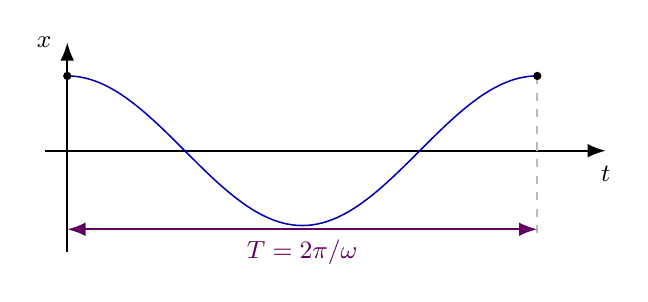
\begin{tikzpicture}[>=Latex, thick, trig format=rad, x=0.95cm, y=0.95cm]
  \draw[->] (-0.3,0) -- (7.2,0) node[below=2pt, font=\small]{$t$};
  \draw[->] (0,-1.35) -- (0,1.45) node[left=2pt, font=\small]{$x$};
  \draw[blue!70!black, smooth, domain=0:2*pi, samples=80, line width=0.55pt]
    plot (\x, {cos(\x)});
  \pgfmathsetmacro{\T}{2*pi}
  \draw[dashed, gray!55] (\T,1) -- (\T,-1.1);
  \fill (0,1) circle (1.5pt);
  \fill (\T,1) circle (1.5pt);
  \draw[<->, violet!75!black] (0,-1.05) -- node[below, font=\small]{$T=2\pi/\omega$} (\T,-1.05);
\end{tikzpicture}
\end{center}

\resultbox{The time for one full cycle of SHM is the period
\[
T=\frac{2\pi}{\omega}.
\]
For a spring--mass oscillator, \(\omega=\sqrt{k/m}\), so \(T=2\pi\sqrt{m/k}\).}

\examplebox{A stiff spring (large \(k\)) shortens the period; a heavier mass
(longer \(m\)) lengthens it.}

\end{document}
